\cleardoublepage

\section{Fuzzing, Operating Systems, and Virtual Machines technology} \label{chap:theory}

This thesis will focus on setting up fuzzing on small, embedded systems. To simulate this environment, the \textit{OPTEE OS} operating system will be used as the platform for the fuzzer. Additionally, I wanted to focus on fuzzing software written in \textit{Rust}, as it is becoming more and more popular in system design. Consequently, this chapter will describe all the relevant topics, starting from the actual fuzzing itself. This will be followed by the analysis of the \textit{QEMU} system emulator, which will be utilized to run the \textit{OPTEE OS}. Since \textit{OPTEE OS} runs under the \textit{ARM Trustzone} technology, it too will be briefly mentioned. In the end, the \textit{Rust} language will be quickly introduced, showing the most interesting features and utilities that will be useful for fuzzing.

\subsection{Fuzzing} 

Creating tests automatically or manually is vital for delivering secure and stable software. However, the task of doing it by hand might be challenging as the complexity rises. At some point, it's not worth spending hours trying to figure out another edge case the tested software may encounter. To solve such issues, automatic test generators or fuzzers were invented. As stated in \cite{fuzzing_state_of_art} fuzz testing or fuzzing in short is a technique that uses invalid data to find bugs and security vulnerabilities. In a nutshell, this process involves taking a sequence of bytes and then passing it as input to the target. Therefore, we can divide this process into two parts, the first being the generation and the latter the interpretation. In the case of, file format parsers like, for example, image viewers, it is rather straightforward as the generated sequence can be passed directly as an image file. On the other hand, fuzzing language interpreters is more sophisticated, as supplying them with random data might not go over the lexical and grammatical part of the parser. As a result, it limits our ability to explore the target. The topic of fuzzing language interpreters was brought up as operating systems and interpreters have in some sense much in common. Both take some language as input and conduct extensive checks on the input. In the case of operating systems, this language consists of a sequence of system calls.


\paragraph{Simplest fuzzing setup}
The simplest fuzzing setup is shown in figure \ref{fig:simp_fuzz}. It consists of a test case generator and the target. To tell the generator what happened with the program after the test case was executed, the program exit code is sent back to the fuzzer. In a typical \textit{POSIX} type system, the generator might use \textit{fork()} to spawn the program and then one of the \textit{wait} functions to check the result. Then, we end up with a generator that's constantly spawning new instances of the target program and then runs a single test case. As already mentioned, this design is easy to implement but has significant performance flaws. When generating the test cases as completely random data, the fuzzer will behave as a random walk search algorithm. In such cases, the search space consists of test cases and the sought solution is the one causing the program to fail. It is known that random walking is asymptotically complete, meaning that given enough time it will find the solution. The only problem is that in most applications it is too slow and will require vastly more resources to achieve the same level of exploration as the more sophisticated algorithms.

\tikzstyle{n} = [rectangle, rounded corners, minimum width=2cm, minimum height=1cm,text centered, draw=black, fill=green!30]

\begin{figure}[h!]
    \centering

    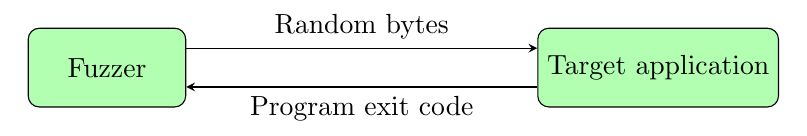
\begin{tikzpicture}[node distance=2cm]
        \node (fuzzer) [n] {Fuzzer};
        \node (app) [n, right of=fuzzer, xshift=5cm] {Target application};
        \begin{scope}[transform canvas={yshift=.7em}]
            \draw [-stealth] (fuzzer) -- node[anchor=south] {Random bytes} (app);
        \end{scope}
        \begin{scope}[transform canvas={yshift=-.7em}]
            \draw [-stealth] (app) -- node[anchor=north] {Program exit code} (fuzzer);
        \end{scope}
    \end{tikzpicture}

    \caption{The easiest fuzzing setup.}
    \label{fig:simp_fuzz}
\end{figure}

\subsubsection{Genetic Fuzzing}

The next step in the evolution of fuzzer programs was the employment of heuristic algorithms to speed the process up. Usually, these were different variations of genetic algorithms, therefore such fuzzers were categorized as genetic or guided. The first fuzzer to use this approach successfully was the \textit{American Fuzzy Loop} developed by Michał Zalewski in \cite{afl}. To see how such a fuzzer works, let us assume that we have some metric allowing us to compare how a single test case generated by the fuzzer is better than the other. Now it is possible to use a genetic algorithm to act as the test case generator. Each specimen is a test case stored as a sequence of bytes. They are mutated using several methods which are specific to each fuzzer. Designing a good mutator requires some experience in testing software. For example, typical memory pitfalls present in languages like \textit{C} or \textit{C++} appear when the index accessing some array becomes a very large or negative number. This if not properly handled leads to out-of-bounds access which can have serious security consequences. With this knowledge, a good way to start is to mutate a single byte in the test case by:
\begin{itemize}
    \item negating it,
    \item exchanging with 255 or \textit{FF} in hex,
    \item exchanging with 0.
\end{itemize}
Furthermore, we can duplicate some fragments of the test case or truncate it. Next, after mutating all specimens, fitness is asserted and those which doesn't meet the succession criteria are discarded. Those that do, are added to the test case set, which is also called fuzzer's corpus. To summarize, in the big picture we only need to add an evaluation method to the previous setup to properly employ a better fuzzing algorithm, as shown in figure \ref{fig:genetic_fuzz}.  

\begin{figure}[h!]
    \centering

    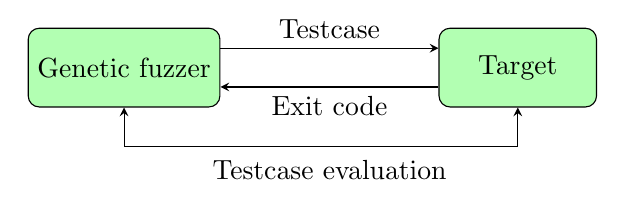
\begin{tikzpicture}[node distance=2cm]
        \node (fuzzer) [n] {Genetic fuzzer};
        \node (app) [n, right of=fuzzer, xshift=3cm] {Target};
        \begin{scope}[transform canvas={yshift=.7em}]
            \draw [-stealth] (fuzzer) -- node[anchor=south] {Testcase} (app);
        \end{scope}
        \begin{scope}[transform canvas={yshift=-.7em}]
            \draw [-stealth] (app) -- node[anchor=north] {Exit code} (fuzzer);
        \end{scope}

        \draw [stealth-stealth] (app) -- ++(south:1cm) -| node[anchor=west, xshift=1cm, yshift=-0.3cm] {Testcase evaluation} (fuzzer);
    \end{tikzpicture}

    \caption{Genetic fuzzer setup.}
    \label{fig:genetic_fuzz}
\end{figure}

\subsubsection{Defining the fitness metric}
Let us assume we have two test cases we want to compare. One possibility for doing that is to see which lines of code were executed in the target program. One such example is shown in listing \ref{lst:tc1} for the first test case and \ref{lst:tc2} for the other. The lines of code which were executed are highlighted in yellow. We can see that the first test case covered 4 out of 7 lines, which yields a code coverage value of $\frac{4}{7}$. The other covered all 7 out of 7 lines, which yields a value of $1$. Apart from numerical results, we can see that the second test case reached a potentially dangerous code fragment. This metric known as code coverage was well tested and used in software engineering processes as early as the 1960s in IBM as referred to in \cite{ibm_coverage}. Furthermore, researchers in \cite{coverage} showed that code coverage is moderate to strongly correlated to test suite effectiveness. At the same time, test suite size was weakly to moderately correlated with its effectiveness. In conclusion, code coverage is a very important and useful metric in the field of software testing as it allows for the security and stability assessment of software.

\begin{minipage}\linewidth
    \begin{lstlisting}[language=C,caption={Code coverage of the first testcase.},label={lst:tc1},captionpos=b]
<@\colorbox{yellow!30}{if (input[0] == 1) \{}@>
    <@\colorbox{yellow!30}{if (input[10] == 0xFF) \{}@>

        if (input[11] - input[12] > input[0])
            memcpy(&input[20], &input[30], input[40]);
    <@\colorbox{yellow!30}{\}}@>
<@\colorbox{yellow!30}{\}}@>
    \end{lstlisting}
\end{minipage}

\begin{minipage}\linewidth
    \begin{lstlisting}[language=C,caption={Code coverage of second testcase.},label={lst:tc2},captionpos=b]
<@\colorbox{yellow!30}{if (input[0] == 1) \{}@>
    <@\colorbox{yellow!30}{if (input[10] == 0xFF) \{}@>

        <@\colorbox{yellow!30}{if (input[11] - input[12] > input[0])}@>
            <@\colorbox{yellow!30}{memcpy(\&input[20], \&input[30], input[40]);}@>
   <@\colorbox{yellow!30}{\}}@>
<@\colorbox{yellow!30}{\}}@>
    \end{lstlisting}
\end{minipage}

\paragraph{Taking measurements}
From the fuzzer point of view, there are no lines of code, only assembly instructions, and addresses. As a result, the final metric must rely only on addresses. From now on, there are two approaches, if the source code is available it can be instrumented during compilation. For clarity, software instrumentation is the process of adding additional instructions to perform a specific action. Usually, it is done to add a new functionality to the source code that didn't exist before. On the other hand, the lack of source code enforces the need to inject instrumentation dynamically during runtime. Formally, the first method is called \textit{whitebox fuzzing} and the latter the \textit{blackbox fuzzing}. In each case, the inserted instrumentation has one goal, to log the total execution path. A correct way of doing this would be to log every address being executed. Of course, taking down each one is unnecessary, as only a branching instruction may change the code block that is being executed. For clarity, a code block is a continuous list of assembly instructions that are executed without any jumps or other control flow instructions. 

One disadvantage of \textit{whitebox fuzzing} in the context of embedded systems is that the added instrumentation will increase the memory requirements for a system. Therefore, sometimes it is easier to fuzz using the \textit{blackbox} technique. In this thesis, an approach similar to that taken by \cite{tracecoverage} can be implemented. In this work, researchers use profiling data from a virtual machine to calculate the coverage value. Of course, a virtual machine in this context refers to the \textit{Java} runtime environment. The authors use the \textit{Just In Time} compiler embedded inside \textit{Java} for code instrumentation. This thesis will focus on the \textit{whitebox fuzzing} approach to simplify the needed instrumentation. It will use a modified \textit{QEMU} to generate messages marking which code blocks were executed.

\subsubsection{AFLplusplus fuzzer} \label{sec:afl}

\textit{AFLpluslus} is an example of a genetic fuzzer that came to life as a result of the work in \cite{AFLplusplus-Woot20}. It was created as a successor to the \textit{AFL} fuzzer which is not developed anymore. All \textit{AFL} family fuzzers to which the \textit{AFLplusplus} belongs have a similar mechanism inside. A simplified diagram of the inner workings can be seen in figure \ref{fig:geneticfuzz}. It consists of the \textit{Input Queue}, which stores test cases for each new-found execution path. Each of them is then mutated to create new test candidates. Those freshly generated test cases are then executed one by one and scored using the gathered coverage data by the injected instrumentation. If the new test case discovers a previously unseen execution path it is added to the input queue, otherwise it is discarded.

\begin{figure}[h!]
    \centering
    \scalebox{1.0}{%
        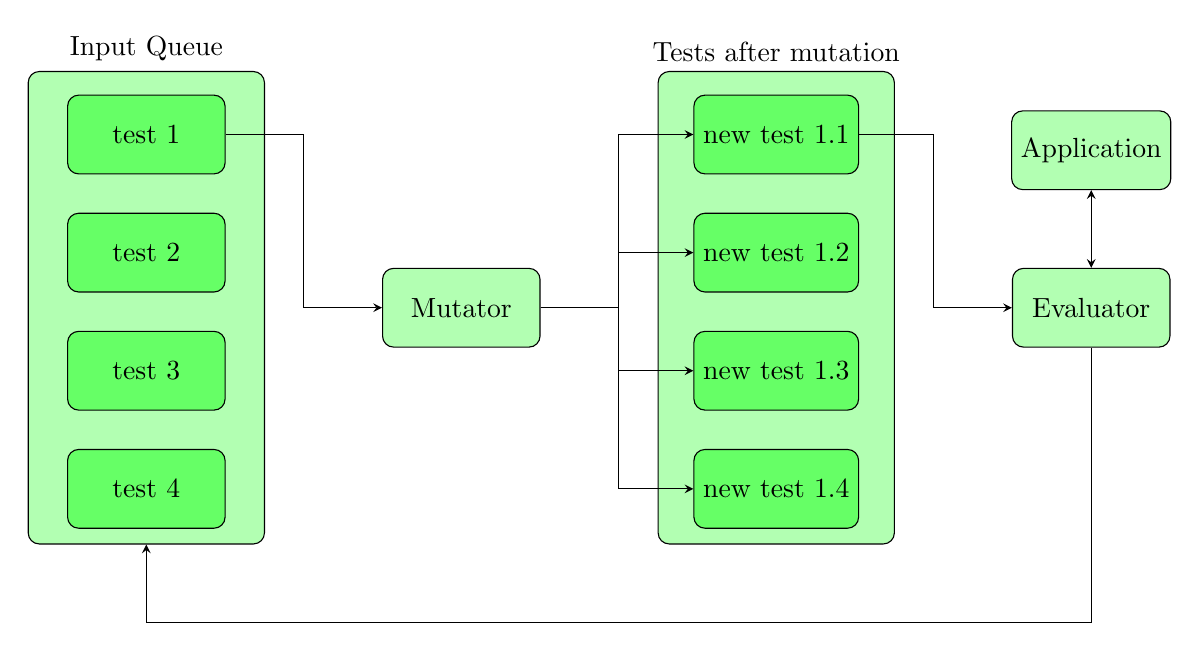
\begin{tikzpicture}
            \node (queue) [n, minimum height=6cm, minimum width=3cm, label=above:{Input Queue}] {};
            \node (test1) [n, fill=green!60, yshift=2.2cm] {test 1};
            \node (test2) [n, fill=green!60, yshift=-0.5cm, below of=test1] {test 2};
            \node (test3) [n, fill=green!60, yshift=-0.5cm, below of=test2] {test 3};
            \node (test4) [n, fill=green!60, yshift=-0.5cm, below of=test3] {test 4};
            \node (mut) [n, right of=queue, xshift=3cm] {Mutator};
            \node (mutqueue) [n, minimum height=6cm, xshift=3cm, minimum width=3cm,
                label=above:{Tests after mutation}, right of=mut] {};
            \node (muttest1) [n, fill=green!60, yshift=3.2cm, below of=mutqueue] {new test 1.1};
            \node (muttest2) [n, fill=green!60, yshift=-0.5cm, below of=muttest1] {new test 1.2};
            \node (muttest3) [n, fill=green!60, yshift=-0.5cm, below of=muttest2] {new test 1.3};
            \node (muttest4) [n, fill=green!60, yshift=-0.5cm, below of=muttest3] {new test 1.4};
            \node (eval) [n, right of=mutqueue, xshift=3cm] {Evaluator};
            \node (app) [n, above of=eval, yshift=1cm] {Application};

            \draw [-stealth] (test1) -- +(east:2cm) |- (mut);
            \draw [-stealth] (mut) -- +(east:2cm) |- (muttest1);
            \draw [-stealth] (mut) -- +(east:2cm) |- (muttest2);
            \draw [-stealth] (mut) -- +(east:2cm) |- (muttest3);
            \draw [-stealth] (mut) -- +(east:2cm) |- (muttest4);
            \draw [-stealth] (muttest1) -- +(east:2cm) |- (eval);
            \draw [stealth-stealth] (app) -- (eval);
            \draw [-stealth] (eval) -- +(south:4cm) -| (queue);
        \end{tikzpicture}
    }
    \caption{Detailed example of a genetic fuzzer.}
    \label{fig:geneticfuzz}
\end{figure}

\paragraph{AFL's instrumentation} \label{sec:aflinstr}
The \textit{AFL fuzzer} requires the injection of code coverage instrumentation, which can be done either by a specially modified version of \textit{gcc} compiler or \textit{QEMU} emulator. In each case, the added code is almost the same and involves invoking the \textit{afl\_maybe\_log} function whenever a new branch is taken. The code of this function from \cite{aflpprepo} can be seen in listing \ref{afl_instr}. In general, this function takes the currently logged address as an argument and proceeds to increment a cell in a hash map. To additionally decrease the collisions, a simple hashing algorithm is employed, as seen in lines 4 and 7. It relies on holding the previous value of the address to mix it with the new one. Moreover, when the current value is assigned to the \textit{afl\_prev\_loc} it is shifted by one to further increase mixing. This might seem strange, as it adds a chain dependency to the sequence of indexes. In a typical hash map, this is unacceptable and results in different results based on the order of accesses. However, this is very beneficial from the standpoint of the fuzzer. One effect of this design is the encoding of how many iterations a loop undertook. Without the chaining, each loop iteration might generate exactly the same index sequence as the previous one. Next, the calculated index is truncated to the hash table size by a logic multiplication in line 5. In the end, the value is used to access and increment the element in the coverage map in line 6. After the test case is finished executing, this table is used to determine if a new execution path was found.

\begin{minipage}\linewidth
    \begin{lstlisting}[language=C,caption={Instrumentation code from AFLPlusPlus fuzzer.},captionpos=b,label={afl_instr}]
    void afl_maybe_log(unsigned long cur_loc) {
    
      if (afl_area_ptr == NULL) { return; }
      unsigned long afl_idx = cur_loc ^ afl_prev_loc;
      afl_idx &= MAP_SIZE - 1;
      INC_AFL_AREA(afl_idx);
      afl_prev_loc = cur_loc >> 1;
    
    }
    \end{lstlisting}
\end{minipage}

\subsubsection{Fuzzing language interpreters}
As it was shown, fuzzing can be as easy as starting the target program, passing some random data as input, and watching what happens. Unfortunately, this is not the case for more complicated software like language interpreters and compilers. What makes such software stand out is its architecture. Each of such programs consists of modules processing the data in a pipeline. On its own, such data processing is not a problem for fuzzers. The issue here is the fact that a failure at any level halts data processing. As a result, passing random data will likely always fail processing at the first stage of the pipeline and hide bugs in later stages. To solve this, researchers created the \textit{Fluff fuzzer} in \cite{dominiak2019efficient} which allowed fuzzing language interpreters more efficiently.

\paragraph{Language interpreters approach}
To handle such sophisticated software, a different approach to preparing input must be developed. For example, researchers in \cite{dominiak2019efficient} suggested generating input using language grammar. Thanks to this, we can ensure that the generated sequences will pass the lexical analysis and most likely also the grammatical one. As a result, the fuzzer will target the deeper layers from the semantic analyzer to the actual interpreter itself. To accomplish this, the \textit{Fluff fuzzer} takes the language's grammar description and uses it to generate random expressions. In detail, each tense in a language can be dissected into a graph based on grammar rules. Therefore, the fuzzer needs to generate random graphs which follow the language's grammar. Let us assume a simplified grammar like that presented in figure \ref{fig:astex}. Here, the program begins with a statement, which then has 3 possible paths. To choose one of them, the fuzzer reads a single byte from the test case and draws the path by dividing it by the number of possibilities and using the remainder as an index. The options from which the fuzzer can select are as follows:
\begin{enumerate}
    \item variable declaration - this statement only depends on one expression which is the assigned value, in this case, the fuzzer can read the variable name from the test case and proceed with the definition of the expression,
    \item expression - this represents a sequence of operations that yield a value, in this simplified example an expression has 4 types:
    \begin{enumerate}
        \item addition,
        \item multiplication,
        \item literal - a numeric value,
        \item division,
    \end{enumerate}
    \item if statement - a simple conditional operator that will execute the body when the condition is true.
\end{enumerate}

\tikzstyle{statement} = [rectangle, minimum width=3cm, minimum height=1cm,text centered, draw=black, fill=green!30]
\tikzstyle{expression} = [rectangle, minimum width=3cm, minimum height=1cm,text centered, draw=black, fill=yellow!30]
\tikzstyle{other} = [rectangle, minimum width=3cm, minimum height=1cm,text centered, draw=black, fill=red!30]
\tikzstyle{arrow} = [thick,->,>=stealth]

\begin{figure}[h!]
    \centering

    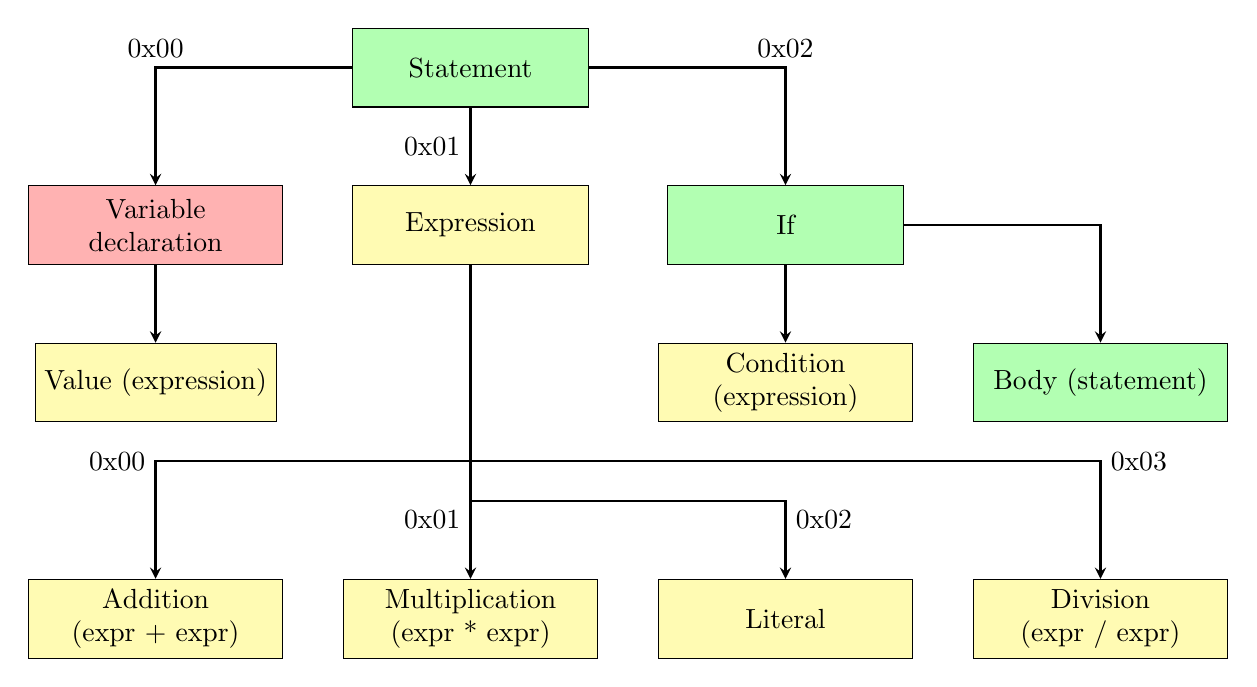
\begin{tikzpicture}
        \node (stmt) [statement] { Statement }; 
        \node (expr) [expression, below of=stmt, yshift=-1cm] { Expression };
        \node (var) [other, left of=expr, xshift=-3cm, text width=3cm] { Variable declaration };
        \node (if) [statement, right of=expr,xshift=3cm] { If };

        \node (expr2) [expression, below of=var, yshift=-1cm] { Value (expression) };

        \node (expr3) [expression, below of=if, yshift=-1cm, text width=3cm, xshift=0cm] { Condition (expression) };
        \node (stmt2) [statement, right of=expr3, text width=3cm, xshift=3cm] { Body (statement) };

        \node (add)  [expression, text width=3cm, below of=expr2, yshift=-2cm] { Addition (expr + expr) };
        \node (mul)  [expression, text width=3cm, below of=expr, yshift=-4cm] { Multiplication (expr * expr)};
        \node (lit)  [expression, text width=3cm, below of=expr3, yshift=-2cm] { Literal };
        \node (call) [expression, text width=3cm, below of=stmt2, yshift=-2cm] { Division (expr / expr) };

        \draw [arrow] (stmt) -| node[anchor=south] { 0x00 } (var);
        \draw [arrow] (stmt) -| node[anchor=south] { 0x02 } (if);
        \draw [arrow] (stmt) -- node[anchor=east] { 0x01 } (expr);

        \draw [arrow] (var) -- (expr2);
        \draw [arrow] (if) -- (expr3);
        \draw [arrow] (if) -| (stmt2);

        \draw [arrow] (expr) --++(0cm, -3cm) -- node[anchor=east] { 0x01 } (mul);
        \draw [arrow] (expr) --++(0cm, -3cm) -| node[anchor=east] { 0x00 } (add);
        \draw [arrow] (expr) --++(0cm, -3cm) -| node[anchor=west] { 0x03 } (call);
        \draw [arrow] (expr) --++(0cm, -3.5cm) -| node[anchor=north west] { 0x02 } (lit);
        
    \end{tikzpicture}
    
    \caption{Simplified grammar example.}
    \label{fig:astex}
\end{figure}

After the syntax tree has been generated, the fuzzer can proceed with code generation. To illustrate this process, let us assume that the tree generated by the fuzzer in the previous step is presented in figure \ref{fig:gentree}. To generate code from a tree, the algorithm must traverse it starting from the deepest nodes and gradually moving up. Each time, the code generator encounters a node, it will yield the code based on the node type and its children which were already processed. For example, all arithmetic operations can yield \textit{(first child) operation (second child)}. Statements are more complicated but in this simplified case they can be compiled as follows:
\begin{itemize}
    \item if statement - can yield \textit{if (condition) { body }},
    \item variable declaration - can yield \textit{var name = (value)}.
\end{itemize}
The generated code for this example can be seen in listing \ref{lst:gensrc}. Of course, this example wasn't made with any programming language in mind and is only provided for explanatory reasons.

\begin{figure}[h!]
    \centering

    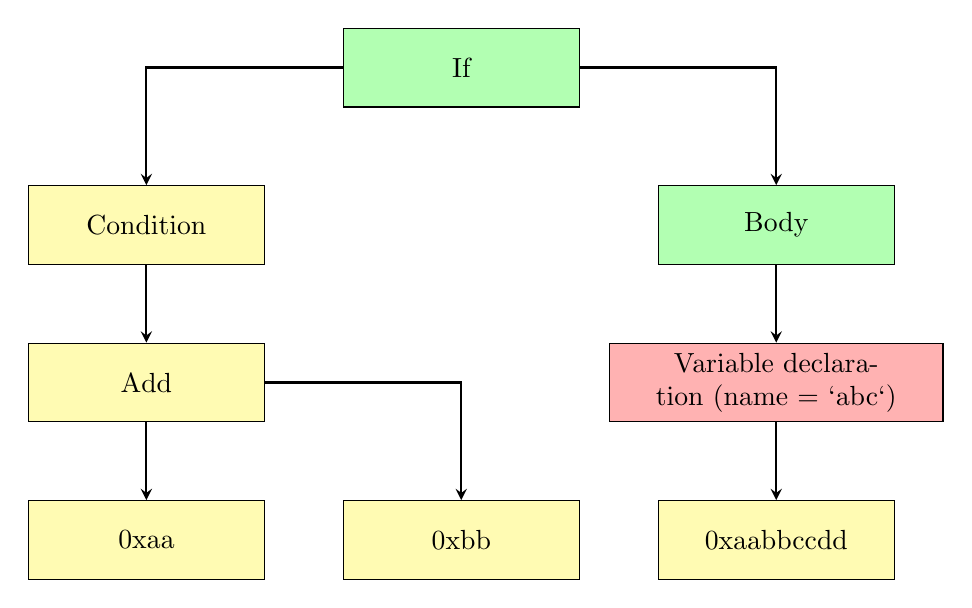
\begin{tikzpicture}
        \node (if) [statement] { If };
        
        \node (cond) [expression, below of=if, yshift=-1cm, xshift=-4cm] { Condition };
        \node (add) [expression, below of=cond, yshift=-1cm] { Add };
        \node (lit1) [expression, below of=add, yshift=-1cm] { 0xaa };
        \node (lit2) [expression, right of=lit1, xshift=3cm] { 0xbb };

        \node (body) [statement, right of=cond, xshift=7cm] { Body };
        \node (var) [other, below of=body, text width=4cm, yshift=-1cm] { Variable declaration (name = `abc`) };
        \node (lit3) [expression, below of=var, yshift=-1cm] { 0xaabbccdd };

        \draw [arrow] (if) -| (cond);
        \draw [arrow] (if) -| (body);
        \draw [arrow] (cond) -- (add);
        \draw [arrow] (add) -- (lit1);
        \draw [arrow] (add) -| (lit2);
        \draw [arrow] (body) -- (var);
        \draw [arrow] (var) -- (lit3);
    \end{tikzpicture}
    
    \caption{Generated syntax tree.}
    \label{fig:gentree}
\end{figure}

%\pagebreak
\begin{minipage}{\linewidth}
\begin{lstlisting}[language=python,caption={Generated program from syntax tree.},label={lst:gensrc}]
if ((0xaa) + (0xbb)) {
    var abc = (0xaabbccdd)
}    
\end{lstlisting}    
\end{minipage}


\subsubsection{Fuzzing Operating Systems}

Fuzzing operating systems have some similarities with fuzzing language interpreters. Firstly, the operating system exposes its \textit{API} to user applications. These system calls, or \textit{syscalls} for short, can be interpreted as a language the application employs to talk to the operating system. Therefore, a good way to fuzz operating systems is to create an application that will communicate with the actual fuzzer and run test cases by calling system calls. For example, the \textit{syscalls} of the \textit{Linux} kernel consists of a function number and a couple of arguments. Those arguments can be either a number, a buffer with data, or a \textit{C} language structure. Thanks to the \textit{Linux} system implementing the \textit{POSIX} standard, the kernel uses a file descriptor to implement a generic identifier for various functionalities. This limits the complexity of the fuzzer. 

\paragraph{Interpreting system calls}
 
Based on those assumptions, researchers have designed many solutions for fuzzing \textit{Linux} operating system. One such fuzzer was the \textit{Syzkaller} from \cite{syzkaller}. It works by employing a specially created language used for describing \textit{syscalls}. The programs written in this Domain Specific Language, or DSL for short, are first generated and then sent to the virtual machine to be interpreted by the \textit{syscall} executor. A program example from \cite{syzkaller_repo} written in this language can be seen in listing \ref{lst:syzkaller_dsl}. Based on this example we can see that the mentioned language looks very similar to \textit{C} but what stands out is the \textit{AUTO} keyword. It is used to allocate an automatically cleaned-up variable, it works as a simple garbage collection. In the provided example, the code is passing a text literal as an argument which requires a pointer. That is why the \textit{AUTO} keyword is used to allocate a buffer with some data and then take a pointer to it. This mechanism will ensure that the buffer is not freed until the pointer is in use during fuzzing. In this program, the arguments of the \textit{openat} function were initialized as follows:
\begin{enumerate}
    \item \textit{int dirfd} - file descriptor pointing to a directory, got value \textit{0xffffffffffffff9c} which is some negative number when converted to an \textit{int},
    \item \textit{const char* pathname} - this argument takes a pointer to a text literal, to initialize it the fuzzer allocated the buffer with the text and acquired a pointer, here it will try to open "./file1",
    \item \textit{int flags} - this specifies how the file will be opened, it is usually provided with a bit mask where each bit is responsible for a special behavior like readability, the value of \textit{0x42} represents a random combination of these bits,
    \item \textit{mode\_t mode} - this is the fourth and optional parameter that specifies access rights, as the previous argument it's a bit mask and is similarly supplied with value of \textit{0x1ff} which is a random combination of them.
\end{enumerate}
Similarly, the \textit{write} function is called with:
\begin{enumerate}
    \item \textit{int fd} - file descriptor to write the data to, here it is the result of \textit{openat} function described above,
    \item \textit{const char *buf} - buffer of data to write, here it is an allocated text literal of value "01010101",
    \item \textit{size\_t size} - the number of bytes to write, here equal to 4.
\end{enumerate}

\begin{minipage}\linewidth
    \begin{lstlisting}[language=C,caption={\textit{Syzkaller} DSL describing syscalls.},captionpos=b,label={lst:syzkaller_dsl}]
# Obtain a file handle
r0 = openat(0xffffffffffffff9c, &AUTO='./file1\x00', 0x42, 0x1ff)

# Perform a write operation
write(r0, &AUTO="01010101", 0x4)
    \end{lstlisting} 
\end{minipage}

\paragraph{\textit{Syzkaller} schematic}

The overview of the \textit{Syzkaller fuzzer} from \cite{syzkaller_repo} is shown in \ref{fig:syz}. It consists of three main modules:
\begin{enumerate}
    \item \textit{syz-manager} - this is the main program managing virtual machines with the fuzzed operating system,
    \item \textit{syz-fuzzer} - the actual fuzzer, it runs the genetic algorithm steps, creating new test cases and sending those which uncovered a new execution path to the \textit{syz-manager},
    \item \textit{syz-executor} - this module does the execution of the test case.
\end{enumerate}
As shown in the diagram, the \textit{syz-manager} is the only module running outside the targeted operating system. It is designed this way to survive the fuzzed kernel failure, as this is the module keeping the corpus. To conserve time, the manager communicates with the fuzzer via RPC and the executor shares a memory region with the fuzzer. This way, time lost between test case executions can be minimal. As for gathering the coverage information, this fuzzer uses the built-in \textit{kcov} mechanism inside the Linux kernel. Of course, this requires the kernel to be compiled with the correct debugging options. Nonetheless, it is rather simple to use. The downside of this method is that we can only fuzz targets with the coverage measuring support built-in.

\begin{figure}
    \centering
    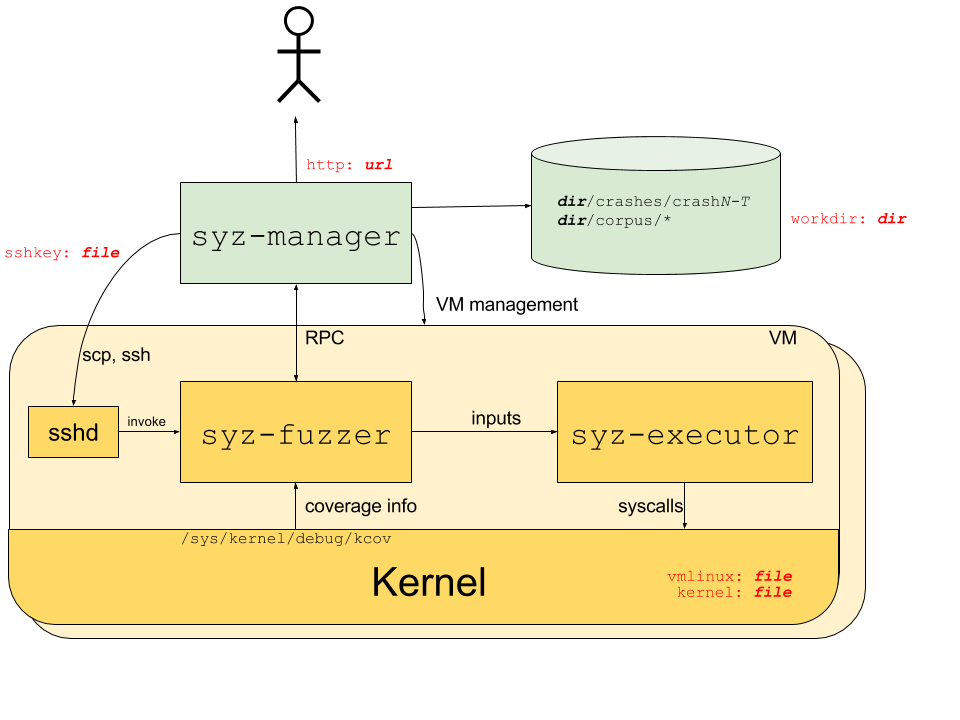
\includegraphics[width=.9\linewidth]{tex/img/syz.png}
    \caption{The diagram of \textit{Syzkaller} fuzzer.}
    \label{fig:syz}
\end{figure}

\subsection{Operating systems and platform emulation}
Operating systems are designed to run on bare hardware without any emulation or virtualization, with direct access to hardware. For this reason, the kernels are heavily reliant on the provided hardware and don't allow for running a second operating system beside them. To address this issue, engineers started creating emulators that were capable of running foreign code and simulating a particular hardware of the emulated architecture. The first \textit{Intel x86} virtual machine managers allowing system emulation were released by \textit{VMWare} in 1999 as stated in \cite{vms}. This was accelerated by the introduction of the \textit{Vt-x} Intel CPU features. This virtualization extension allowed for hardware acceleration of processor emulation. In detail, it provides isolation between emulated and physical processors, so the virtual machine manager only needs to manage the emulated hardware. This improvement eliminated the need to emulate CPU instruction in the emulator's code, thereby making the virtual machine run almost as fast as the host. Of course, since \textit{Vt-x} is a processor extension, this didn't simplify emulating hardware inside a virtual machine, and the virtual machine manager is still required to either fully emulate a virtual component or pass through the real ones from the host. 

Later, the \textit{QEMU} or the \textit{Quick EMUlator} project was created at \cite{qemurepo}. It allowed for easy emulation of various hardware and processor architectures. As a result, \textit{QEMU} has a sophisticated architecture consisting of several modules and platform descriptions. Each platform represents an emulated hardware, it can be chosen from a variety of types from a generic Intel x86 to a very specific embedded ARM CPU or even some old architectures like SPARC.

\subsubsection{QEMU emulator architecture}

Emulating operating systems requires simulating the CPU as well as the hardware. To accomplish this, \textit{QEMU} employs various techniques. Firstly, to emulate the CPU, we have the choice between hardware-accelerated virtualization and full software emulation. The acceleration uses features built into the CPU to provide isolation between virtual machines and the host. The disadvantage is that it only works when the emulated processor is of the same architecture. To simulate an incompatible processor, every instruction needs to be simulated in software. Such translation is similar to, for example, how a \textit{JIT} compiler operates. The module in \text{QEMU} responsible for that is called the \textit{Tiny Code Generator}, or simply the \textit{TCG}. For clarity, all described below components have been put in a diagram available in figure \ref{fig:qemuarch}.

\tikzstyle{qemu} = [rectangle, minimum width=3cm, minimum height=1cm,text centered, draw=black, fill=green!10]
\tikzstyle{thread} = [rectangle, minimum width=3cm, minimum height=1cm,text centered, draw=black, fill=orange!30]
\tikzstyle{module} = [rectangle, text width=2cm, minimum height=1cm,text centered, draw=black, fill=yellow!30]
\tikzstyle{darrow} = [thick,<->,>=stealth]

\begin{figure}[h!]
    \centering

    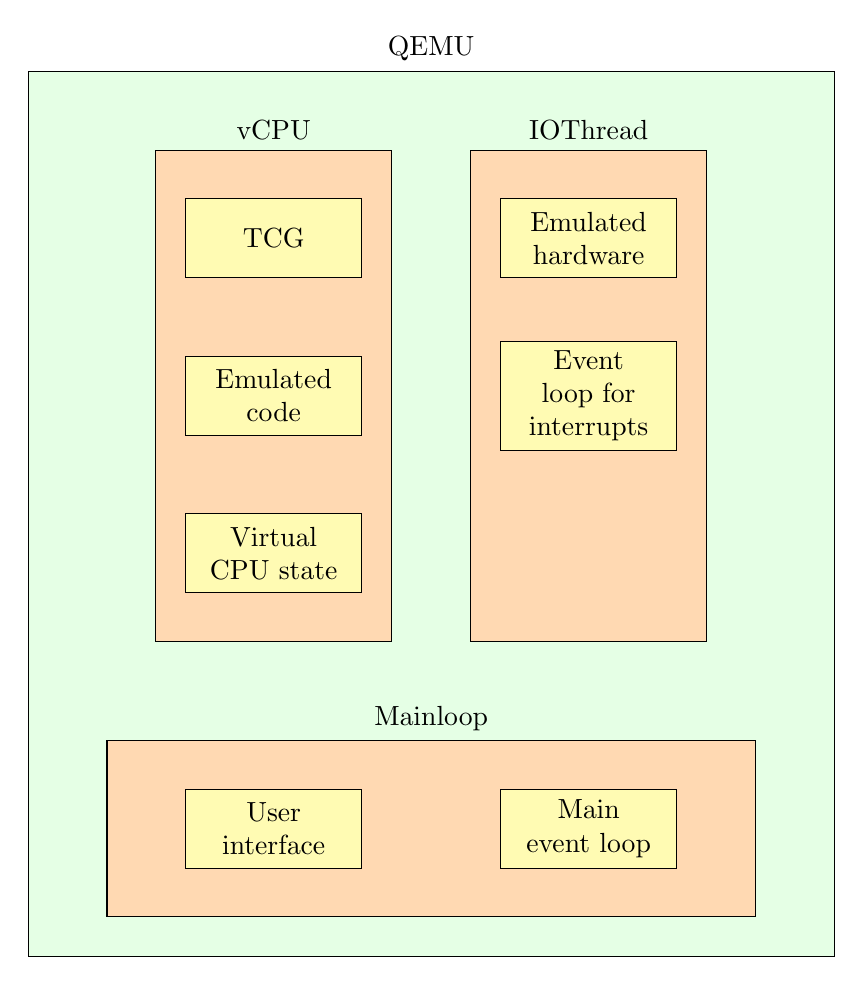
\begin{tikzpicture}
        \node (qemu) [qemu, text width=10cm, text height=11cm, label=north:QEMU] {};

        \node (main) [thread, yshift=-4cm, text width=8cm, text height=2cm, label=north:Mainloop] {};
        \node (vcpu) [thread, text width=2cm, text height=6cm, yshift=1.5cm, xshift=-2cm, label=north:vCPU] {};
        \node (iothread) [thread, text width=2cm, text height=6cm, yshift=1.5cm, xshift=2cm, label=north:IOThread] {};

        \node (tcg) [module, xshift=-2cm, yshift=3.5cm] { TCG };
        \node (code) [module, below of=tcg, yshift=-1cm] { Emulated code };
        \node (state) [module, below of=code, yshift=-1cm] { Virtual CPU state };
        \node (io) [module, xshift=2cm, yshift=3.5cm] { Emulated hardware };
        \node (ioevent) [module, below of=io, yshift=-1cm] { Event loop for interrupts };
        \node (user) [module, yshift=-4cm, xshift=-2cm] { User interface };
        \node (event) [module, right of=user, xshift=3cm] { Main event loop};

    \end{tikzpicture}
    
    \caption{QEMU architecture diagram.}
    \label{fig:qemuarch}
\end{figure}


\pagebreak
\paragraph{\textit{Tiny Code Generator}}
The \textit{TCG} module, as described in \cite{qemutcg}, can be split into two parts. The former is translating the emulated CPU instructions into a virtual intermediate assembly called \textit{QEMU OPS}. The latter is translating the intermediate code into host architecture. This design allows for robustness as every supported architecture can be emulated on all of them. This also adds the possibility to modify, that is, instrument the running code at runtime. Additionally, this allows for extending the simulated instruction set by adding new encodings or modifying existing instructions.

The \textit{QEMU OPS} virtual architecture implements a \textit{RISC} like processor with simple load, store, and arithmetic operations. This is of course insufficient to simulate all complicated instructions of a \textit{CISC} processor for example Intel x86. Therefore, the designers of \textit{QEMU} implemented a mechanism allowing to just register a callback function to be run when the translated instruction is executed. This is a very powerful mechanism, as the callback has access to both the emulated system and the \textit{QEMU} process running on the host. This allows not only emulating very complicated instructions of a \textit{CISC} processor but also instruction used to communicate directly with the emulator. Such instructions are called \textit{hyper calls} since they are used in communication with the \textit{hypervisor}.

An example of an intermediate assembly is shown in listing \ref{lst:tcgir} which shows an example list of instructions from \cite{qemutcgir}. It can be seen that most of the instructions are of arithmetic type that can operate on registers and a couple of special ones to interact with memory or QEMU internals. In the end, there are several interesting orders:
\begin{itemize}
    \item \textit{qemu\_st\_i32 r0,tmp0,beul,3} - this is the memory access operation that stores data (from \textit{r0}) on address (\textit{tmp0}), the next 2 arguments specific the access type (endianess, bus width) and memory index which selects kernel and user memory, naturally there exists an equivalent \textit{qemu\_ld\_i32} load instruction,
    \item \textit{call        store\_msr,\$0,tmp0} - this will call the \textit{store\_msr} TCG helper which is a function complied into QEMU, here \textit{\$0} represents the return value and then follows the parameter list,
    \item \textit{set\_label   \$L0} - this instruction is used to assign a label to the current address which can later be used as arguments in branching,
    \item \textit{exit\_tb     \$0x7f5a0caf8043} - this is a special opcode that exists from the translated code to QEMU, it will return to the translation unit which will proceed with the preparation of the next code block.
\end{itemize}
Later in this thesis, chapter \ref{chap:qemu} will focus on modifying this module to allow communication between the \textit{AFL} fuzzer and the operating system running inside.

\begin{minipage}{\linewidth}
\begin{lstlisting}[caption={QEMU TCG intermediate assembly code.},label={lst:tcgir}]
0xfff00100:  movi_i32    r1,$0x10000

0xfff00104:  movi_i32    tmp0,$0x409c
             or_i32      r1,r1,tmp0

0xfff00108:  movi_i32    r0,$0x0

0xfff0010c:  movi_i32    tmp1,$0x4
             add_i32     tmp0,r1,tmp1
             qemu_st_i32 r0,tmp0,beul,3

0xfff00110:  movi_i32    nip,$0xfff00114
             mov_i32     tmp0,r0
             call        store_msr,$0,tmp0
             movi_i32    nip,$0xfff00114
             exit_tb     $0x0
             set_label   $L0
             exit_tb     $0x7f5a0caf8043
\end{lstlisting}
\end{minipage}

\paragraph{\textit{Thread structure}}
To run the virtual machine \textit{QEMU} uses different threads to do different tasks, as described in \cite{qemuthreads}. The main thread called the \textit{Mainloop} is responsible for controlling the emulated machine. It exposes an interface for scheduling tasks and controls the main event loop. All tasks requiring the virtual machine to be in a consistent state are executed in the context of the \textit{Mainloop} thread. The reason is that this thread can halt and shut down other threads when needed. Consequently, scheduled tasks can operate on a synchronized state of all virtual CPUs. One such task is responsible for taking or restoring a snapshot. While the virtual machine is saved, all other threads are suspended and resumed after the operation is finished. Furthermore, the \textit{Mainloop} is also responsible for handling the user interface known as \textit{QEMU monitor}. It allows for controlling the virtual machine from the command line.

Next, to emulate the hardware and interrupts, \textit{QEMU} uses a separate thread called the \textit{IOThtread}. It is also an event loop, but this time it is processing events from emulated hardware. There might be many such threads, but for small systems like embedded processors, one is usually enough. Suspending this thread is essential to ensure that the virtual hardware can be safely inspected and operated on from the outside.

Last, but not least, there are the \textit{vCPU} threads. These are responsible for the described instruction translation and then execution. In the beginning, the emulated assembly code is split into parts called basic blocks. Each block is then translated using the \textit{TCG} module to host machine code. It is stored in an executable memory region. After the translation, \textit{QEMU} starts executing the generated code by simply jumping to it. To speed this process up, \textit{TCG} caches translated blocks so as not to recompile the same fragments many times over. 



\subsubsection{\textit{Trustzone} technology} \label{sec:tz}
All contemporary \textit{CPU} architecture implements a module responsible for providing security features, which is isolated from the main operating system. This way, application developers can create more secure services. Each service can store secrets inside encrypted secure memory or derive keys for encryption and signature verification. Thanks to this, the compromise of the main operating system might not lead directly to the leakage of sensitive data. In \textit{ARM} CPU, this technology is implemented as a more privileged mode of the CPU. It is named \textit{Trustzone} and defined in \cite{trustzonedoc}.

\begin{figure}
    \centering
    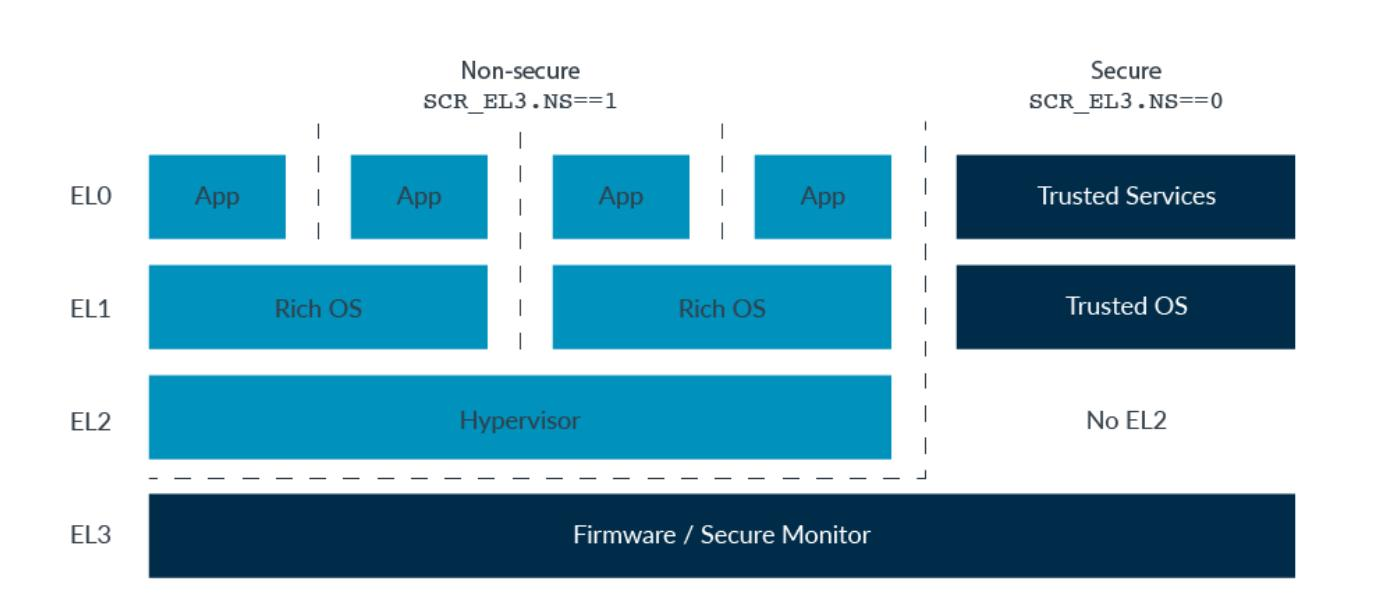
\includegraphics[width=.9\linewidth]{tex/img/trustzone.jpg}
    \caption{Example \textit{Trustzone} implementation in \textit{armv8} architecture.}
    \label{fig:tzarmv8}
\end{figure}

The diagram showing the security architecture of \textit{armv8} processor from \cite{tzsyf} is shown in figure \ref{fig:tzarmv8}. The major difference between this architecture and, for example, the \textit{Intel x86} is the existence of other so-called \textit{worlds}. There is a non-secure world, where the "normal" operating system, like for example \textit{Android} lives. The latter called the secure world provides space for the special security-oriented operating system. On the architectural level, the worlds are implemented by selectively allowing and forbidding access to parts of physical memory based on whether the CPU is running in secure or normal mode. The non-secure world is sometimes called the rich world, as it doesn't implement this many security enhancements as the secure one.

Apart from different worlds, the CPU employs different privilege modes to separate running code. There exist four different levels:
\begin{enumerate}
    \item \textit{EL0} - the least privileged one, all applications run here,
    \item \textit{EL1} - the level on which the operating system runs,
    \item \textit{EL2} - \textit{hypervisor} level, it is used to manage virtual machines running in non-secure mode,
    \item \textit{EL3} - the secure monitor mode, it is responsible for providing separation between worlds and communication with hardware.
\end{enumerate}

\subsubsection{OPTEE OS}
\textit{OPTEE OS} is an open source, security-oriented operating system designed specially for \textit{Trustzone} technology. It consists of a core written in \textit{C} and applications called \textit{Trusted Application} or in short “TA's”. Each such application can expose an interface to either another \textit{TA} or as a service in the non-secure world. The architecture diagram of \textit{OPTEE OS} from \cite{opteeblog} can be seen in figure \ref{fig:optee}. As we can see from the diagram, \textit{OPTEE OS} kernel and application live solely in the secure world and talk to the non-secure through a communication channel provided by the \textit{CPU}. The non-secure world then utilizes a device driver to call secure services. The tasks of such operating systems are wide and range from verifying code signatures through key derivation to storing data securely in encrypted memory. An example of how this technology can be used is provided in \cite{opteeusage}. There, the researchers describe developing security mechanisms useful in \textit{IoT} or \textit{Internet of Things} devices. The article focuses on different aspects of security:
\begin{enumerate}
    \item Confidentiality - making sure that the stored information is available only to authorized appliances, 
    \item Integrity - attesting data and software to detect malicious tampering,
    \item Authorization - to perform security check on the system,
    \item Availability - ensure that the security module is always available,
    \item Privacy - the need to keep all information confidential.
\end{enumerate}
\begin{figure}[h!]
    \centering
    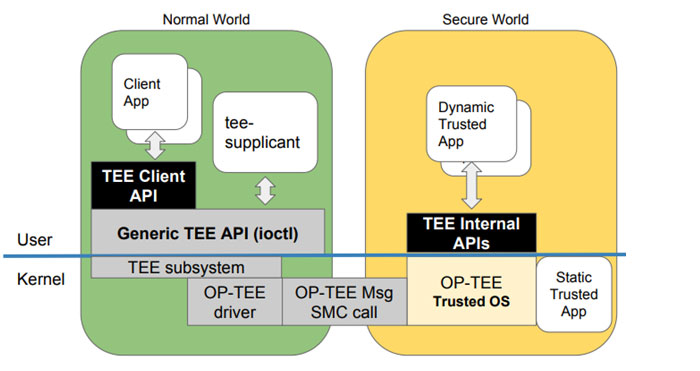
\includegraphics[width=.8\linewidth]{tex/img/op-tee-software-architecture.jpg}
    \caption{\textit{OPTEE OS} architecture diagram.}
    \label{fig:optee}
\end{figure}

\paragraph{\textit{OPTEE OS} architecture}
As a result of \textit{OPTEE OS} being a secure-oriented OS, its application interface provides a lot of cryptography-related functions. It implements many symmetric and asymmetric ciphers along with hash functions. Though the system doesn't implement a casual file system, it has secure encrypted storage that can be accessed from the non-secure world. This allows for creating an application with a special secure part running in \textit{Trustzone} which handles all sensitive operations. Of course, the security of the entire system relies on the security of the secure driver. If there is any vulnerability inside, it may compromise the secure service. Naturally, this is not easy as one must find first a vulnerability in the non-secure application to even reach the secure part, so the isolation adds a level of complexity to a potential attack. As an open source project, \textit{OPTEE OS} can be deployed on a couple of hardware platforms, such as the \textit{Raspberry Pi} family and other boards having an \textit{ARM} CPU with \textit{Trustzone} support. Thankfully, it can also be emulated in \textit{QEMU} using the default \textit{ARM} virtual machine board definition. This makes testing and development easy as it is not required to acquire some special proprietary hardware.



\subsection{Rust programming language and environment}

\textit{Rust} programming language is a recently created, primarily targeted for system programmers. The design of this language is available in so-called \textit{Rust book} in \cite{rustbook}, which is a comprehensive description of features and design choices.  It is advertised as a \textit{C/C++} successor in the fields of operating systems, driver, and operating system services development. Therefore, \textit{Rust} supports many architectures and operating systems. Additionally, it can be compiled without any external dependencies, or in a so-called bare metal environment, to be used to implement the operating system. As with every modern programming language, Rust comes with its package manager. Typically a package manager is a tool allowing for fetching and configuring the dependencies required to compile the project. A project is a directory containing a package. Continuing, a package is a set of crates, and a crate is according to the \textit{Rust} documentation the smallest amount of code that the \textit{Rust} compiler considers at the time. Such an entity consists of the crate manifest and source files. The Rust designers have also divided crates into two types, there can be library crates which can only expose functionalities, and executable crates which are then compiled into a binary.

\paragraph{Advantages of Rust}
\textit{Rust} introduces new security mechanisms which are absent in the family of languages derived from \textit{C}. Primarily, \textit{Rust} focuses on memory and thread safety as stated in \cite{rustmemorysafety}. First, \textit{Rust} abandons the use of pointers and allows only references. This enhancement is motivated by the fact that most bugs found in software are memory corruptions. Along with disallowing the use of pointers inside the so-called safe code, \textit{Rust} introduces lifetime checking of references. The entity enforcing those rules was named the borrow checker, its task is to ensure that all entities live in memory as long as they are used. This eliminates other memory bugs such as the popular “use-after-free” where an object is destroyed, yet there still exists a reference to the freed memory and other parts of the program are still executing as if the object still existed. 

An example of such code can be seen in listing \ref{lst:badcpprust} written in \textit{C++} and \textit{Rust}. In both cases, the function creates a local variable on the stack named \textit{var} and assigns a value of 0. Then the code takes a reference to \textit{var} and returns it from the function. This results in accessing unallocated memory, as the variable is allocated at the beginning of the function and freed just before returning. 

%In comparison, listing \ref{badrust} shows the equivalent code in \textit{Rust}. 
%Here, just like in the \textit{C++} example, the code allocates on the stack a 32-bit signed variable and assigns a value of $0$. Then it proceeds with returning a reference to it. For clarity, in \textit{Rust} the value of the last expression in a function is treated as the return value. Hence, there is no need to explicitly use the \textit{return} keyword, although \textit{Rust} supports it. 

As expected, the \textit{C++} example compiled without issue, only emitting a warning that can be silenced. In the case of Rust, the compiler would terminate the compilation with a message stating that the return value doesn't live long enough as its lifetime is bound to the functions that created it. Additionally, \textit{Rust} controls how references to variables are created. The language introduces two types of references: the immutable one which doesn't allow for the modification of the object it is pointing to, and the mutable which does. There are two major rules governing the creation of these references:
\begin{enumerate}
    \item an object can have immutable references if and only if it doesn't have any mutable reference,
    \item an object cannot have multiple mutable references.
\end{enumerate}
These restrictions ensure that objects don't suddenly change or become deleted while other objects still use them.

Apart from that, \textit{Rust's} assignment operation moves the argument instead of copying it, as is the case in languages like \textit{C++}. This allows to write efficient code, as each copy operation needs to be explicitly allowed. Besides that, the language provides a mechanism to securely pass entities between threads. Basically, \textit{Rust} bans the usage of an object in a multithreaded environment if it doesn't implement the proper synchronization mechanisms. This eliminates race conditions where threads race for access to a shared resource and different order of accesses leads to different execution results. Unfortunately, this doesn't solve the problem of two threads locking up on a shared pair of resources, stalling the execution forever. Therefore, the deadlock problem is still persistent and needs to be avoided. 

\begin{table}
    \centering
    \begin{tabular}{c@{\hskip 1cm}|@{\hskip 1cm}c}
        \begin{lstlisting}
int& function() {
    int var = 0;
    return &var;
}
        \end{lstlisting} &
        \begin{lstlisting}
fn function() -> &i32 {
    let var = 0i32;
    &var
} 
        \end{lstlisting}\\
    \end{tabular}
    \captionof{lstlisting}{Example of a memory corruption bug in C++ and Rust.}
    \label{lst:badcpprust}
\end{table}

\textit{Rust} designers have also abandoned the use of inheritance as a polymorphism mechanism, they instead introduced traits. Each trait defines an interface that can be implemented by a struct, which then allows the object to be referred to as a reference to the trait it implements. This effectively replaces the inheritance, without the potential complications that can arise like, for example, diamond inheritance. For clarity, this class derivation scheme happens when some base class exists in multiple instances in the inheritance tree. Normally, this situation is impossible in languages like \textit{C\#} or \textit{Java} where a class can only inherit from a single base class. As a result, all inheritance schemas are trees, usually starting from a single base class. However, \textit{C++} language allows for multi-base inheritance, which can lead to complicated structures in the derivation graph.

%The simplest diamond inheritance case is shown in figure \ref{fig:dinher}. 

%\begin{figure}[h!]
%    \centering
%
%    \begin{tikzpicture}
%        \node (A) [module] { A };
%        \node (B) [module, below of=A, xshift=2cm, yshift=-1cm] { B };
%        \node (C) [module, below of=A, xshift=-2cm, yshift=-1cm] { C };
%        \node (D) [module, below of=A, yshift=-3cm] { D };
%
%        \draw [arrow] (A) -| (B);
%        \draw [arrow] (A) -| (C);
%        \draw [arrow] (B) |- (D);
%        \draw [arrow] (C) |- (D);
%    \end{tikzpicture}
%    
%    \caption{Diamond inheritance graph example}
%    \label{fig:dinher}
%\end{figure}

%The only limitation that is imposed on what trait can be implemented for which type is that one may not implement a foreign trait for a foreign type. The word foreign means here an entity outside the crate that is providing the trait's implementation. This is done, to not allow for extending external types with new implementation. We might imagine that if this was the case, this could result in many incompatible implementations which would break the project.

\paragraph{Unsafe code}
Sadly, while creating an operating system, this security rules cannot be upheld for the entire code base. Just like stated in \cite{rusthowunsafe}, there are situations where the security checks need to be disabled for a part of the code. Almost all such cases involve talking to computer hardware. Currently, the hardware still has an ugly interface requiring the use of pointers, buffers, and flags or status codes. This, of course, violates the \textit{Rust}'s security rules. Therefore, while developing the code which directly accesses the hardware, some restrictions must be lifted. This is done using the \textit{unsafe} keyword, which defines a code block or a function where \textit{Rust} allows pointers and doesn't check whether the memory is properly managed. Inside those blocks, tasks like memory management and thread synchronization once again rely fully on the programmer. As a result, this might introduce bugs and security vulnerabilities as shown in \cite{rustunsafeissues}, which the designers of Rust want to eliminate. Therefore, the usage of unsafe code should be limited only to required cases and thoroughly reviewed. An example of such a use case is shown in listing \ref{unsafe_rust}. As can be seen, the code defines a variable holding an address to a memory-mapped register. This is a perfectly safe operation as it is just assigning an integer value. However, the next operation violates the security rules. In the next 3 lines, the address will be cast from an integer to an unsigned \textit{int} pointer and then dereferenced. From these two actions, only the dereferencing is unsafe and needs to be enclosed with an \textit{unsafe} block. The reason for it being unsafe is that the \textit{Rust} compiler cannot assert whether this pointer is valid, as it was just converted from an arbitrary numerical value. 

\begin{minipage}{.9\textwidth}
    \begin{lstlisting}[language=rust,caption={Unsafe code example.},captionpos=b,label={unsafe_rust}]
fn read_register() -> u32 {
    let address = 0x20000020 as u32;
    unsafe {
        *(address as *const u32)
    }
}        
    \end{lstlisting}    
\end{minipage}

\subsubsection{Macros and procedural macros}
\textit{Rust} programming language lacks the usual meta programming tools like:
\begin{itemize}
    \item text preprocessor, as in \textit{C}
    \item templates engine as in \textit{C++}, although Rust does have generics, they aren't as powerful as those in \textit{C++}.
\end{itemize}
As a result, \textit{Rust} language designers created another, even more capable mechanism named macros. Instead of extending what generics can do as it happened in the case of \textit{C++}, the designers came up with a tool processing tokens from the source code. It is far superior to a simple text processor, as it can distinguish entities based on \textit{Rust}'s syntax and not only raw text. At the same time, it is way easier to employ than \textit{C++} template system as these macros take as input a stream of tokens which can be matched into different patterns and output another stream of tokens without the need to spend hours trying to code everything functionally using \textit{C++} templates. 

Sometimes a simple macro processing sequence of tokens is not enough. The macros discussed up to this point are declarative structures that are allowed to match patterns and generate code using a simple template metalanguage. Unfortunately, they are not allowed to call functions, allocate variables, or store any type of internal state. For this reason \textit{Rust} introduced the so-called procedural macros. These are essentially functions processing and returning tokens. They are compiled first during the build process and are invoked by the compiler to generate code which will be compiled along with the rest of the source code. What makes such macros powerful is the lack of limits on what can they do. It can even make an internet connection to download some code and add it to the compiled binary. This allows for a huge variety of things that can be done during compile time. However, what is most interesting is the ability to extend the Rust compiler with procedural macros allowing it to transpile some language into \textit{Rust}. Thanks to this the programmers can develop custom languages and seamlessly incorporate them into \textit{Rust}.

To shed some light on \textit{proc macros}, a simple example can be seen in listing \ref{lst:procmacrodef}. It starts with a special attribute \textit{\#[proc\_macro]} which tells the \textit{Rust} compiler that it should treat the function below as a \textit{proc macro}. Like every such macro, the \textit{implement\_magic} takes a \textit{TokenStream} object as argument and returns a \textit{TokenStream}. In detail, the \textit{TokenStream} struct represents the \textit{Rust} compiler's token stream. The function then takes a text literal with \textit{Rust} code inside, which defines a function named \textit{magic}, and converts it to \textit{TokenStream} by calling the \textit{parse()} member function. Finally, these tokens are returned, as this is the last expression in the function's body. The \textit{proc macros}, like the described one, can be later used in another crate, as shown in listing \ref{lst:procmacrousage}. There, the \textit{main} function calls the \textit{magic} function, which doesn't appear to be defined anywhere. However, above the definition of \textit{main} the \textit{implement\_magic} macro is invoked. After the macro finishes executing, the call place is replaced with the tokens from its return value. It defines \textit{magic} function in this case.

\begin{minipage}{\linewidth}
\begin{lstlisting}[language=rust,caption={Example of a \textit{proc macro} definition.},label={lst:procmacrodef}]
#[proc_macro]
pub fn implement_magic(tokens: TokenStream) -> TokenStream {
    "fn magic(x: u32) -> u32 { 0xAA * x + 1 }".parse().unwrap()
}
\end{lstlisting}
\end{minipage}

\begin{minipage}{\linewidth}
\begin{lstlisting}[language=rust,caption={Example usage of a \textit{proc macro}.},label={lst:procmacrousage}]
implement_magic!();

fn main() {
    println!("x = {}", magic(1));
}
\end{lstlisting}
\end{minipage}

\subsubsection{Creating compiler using \textit{syn} and \textit{quote} crates}
As discussed above, procedural macro allows for an easy creation of what is essentially a compiler inside \textit{Rust} compiler. To aid in this task, \textit{Rust} provides the \textit{syn} and \textit{quote} create, which can be used for parsing input and generating output. The \textit{syn} crate contains everything required to parse \textit{Rust} code, along with interfaces to create custom entities and tokens. This crate provides the \textit{Parse} trait which, when implemented, allows the \textit{Rust} compiler to treat it as if it were a part of the language. After the successful parsing, we are left with the syntax tree. The next step is to proceed to the code generation step. Here the language helps by providing the \textit{quote} macro. It is a helper allowing for the construction of a token stream from \textit{Rust} code. A very simple use of those crates can be a macro adding tracing to the program. In listing \ref{proc_macro} we can see a macro that rewrites its argument by adding a line that prints the function's name. It starts with parsing the input as \textit{ItemFn} which represents a function in the \textit{Rust}'s syntax tree. This struct holds all relevant information about a function:
\begin{enumerate}
    \item \textit{attrs} - this array holds all function attributes, these can be other macros or compiler-defined special statements,
    \item \textit{vis} - this is the visibility attribute which can take 3 values: public, private, or inherited,
    \item \textit{sig} - the function's signature, it holds the label, generic parameters, and function's arguments with their definition along with the return value type,
    \item \textit{block} - this array holds a list of statements from the function's body.
\end{enumerate}
All these fields are then in line 4 extracted from the \textit{ItemFn} struct and in the following 2 lines just for convenience two references to the name and list of statements are taken. In the end, the \textit{add\_trace} function generates code using the \textit{quote} macro. This macro is provided with specially augmented \textit{Rust} code. It can be seen that some identifiers are preceded with \textit{\#} or \textit{\#(\# )\*}, these are part of the special language \textit{quote} macro employs. These two attributes mean the following:
\begin{itemize}
    \item a single \textit{\#} before a variable's name will replace its occurrence with its tokenized value, for example, if a variable holds a text literal it will be tokenized as this literal enclosed in double quotes,
    \item the \textit{\#(\#variable)\*} notation assumes that the variable is an array and will repeat what's inside the parenthesis for each element of the array.
\end{itemize}
All these actions are taken to rewrite the function and add a \textit{println} statement at the beginning of this function's body. It can be seen that the attributes and the visibility are rewritten without modification. Then inside the body, a \textit{println} statement is added which prints the function's name. Next follows the expanse of the statements list. Since the additional line is added at the beginning, it doesn't have any impact on the return value.


\begin{minipage}{.9\textwidth}
    \begin{lstlisting}[language=rust,caption={A procedural macro example.},captionpos=b,label={proc_macro}]
#[proc_macro]
pub fn add_trace(item: TokenStream) -> TokenStream {
    let input: ItemFn = parse_macro_input!(item);
    let ItemFn { attrs, vis, sig, block } = input;
    let name = &sig.ident;
    let stmts = &block.stmts;
    quote! {
        #(#attrs)* #vis #sig {
            println!("TRACE {}", #name);
            #(#stmts)*
        }
    }
}
    \end{lstlisting}
\end{minipage}

\paragraph{\textit{SSA} compiler} \label{ssadec}
Designing a compiler is a very challenging and technically complicated task. As a result, researchers studied this field and came up with various approaches designed to simplify all the required compilation steps. One such design is the \textit{Static Single Assignment} or \textit{SSA} in short. As described in \cite{ssabook}, this method restricts how variables can be used. In a nutshell, whenever an assignment operation is taking place, a new variable shall be allocated. This simplifies the optimization algorithms, as now each value of a variable can be symbolically expressed as a tree of operations. It helps the compiler deduce properties of expressions. An example showing the differences between a code written without the rules of \textit{SSA} can be seen in listing \ref{code_1} and that in \textit{SSA} form in \ref{code_2}. It can be seen that in the non \textit{SSA} form the \textit{x} variable is assigned twice, therefore its value may change between lines 2 and 4. As a result, there is no single and simple symbolic expression for the value assigned to label \textit{x}. On the other hand, the \textit{SSA} compatible form example does assign a new label to the \textit{x} variable in line 3. Therefore, it is easier to see how values depend on each other. Additionally, it is beneficial in the context of creating a compiler macro like described above. Since \textit{Rust} forbids taking multiple mutable references to a variable or any immutable whenever a mutable reference exists, keeping everything constant and just reallocating values makes the design already compliant with the language rules. For this reason, this representation will be used in the code generator part of the compiler designed in chapter \ref{chap:envir} in this thesis.

\begin{minipage}{.4\textwidth}
    \begin{lstlisting}[language=C,caption={Code example containing assigments.},captionpos=b,label={code_1}]
<@$x$@> = 1
<@$y$@> = <@$x$@> + 2
<@$x$@> = 4
<@$z$@> = <@$x$@> + 2
    \end{lstlisting}
\end{minipage}
\hfill\vline\hfill
\begin{minipage}{.4\textwidth}
    \begin{lstlisting}[language=C,caption={Code example in SSO notation.},captionpos=b,label={code_2}]
<@$x_0$@> = 1
<@$y_0$@> = <@$x_0$@> + 2
<@$x_1$@> = 4
<@$z_0$@> = <@$x_1$@> + 2
    \end{lstlisting}    
\end{minipage}
